\documentclass[12pt,a4paper]{report}
\usepackage{graphicx}
\usepackage[utf8x]{inputenc}
\usepackage[turkish]{babel}
\usepackage{fullpage}
\usepackage{multirow}

\begin{document}

\begin{center}


\includegraphics{comu-head.png}

\bfseries
\large
T.C.

ÇANAKKALE ONSEKİZ MART ÜNİVERSİTESİ
MÜHENDİSLİK MİMARLIK FAKÜLTESİ
BİLGİSAYAR MÜHENDİSLİĞİ BÖLÜMÜ \\[5.5cm]
OTEL REZERVASYON SİSTEMİ \\[4.5cm]

\normalsize
\it

Mesutcan Kurt    080401013

Orçun Avşar      060401007 \\[2.4cm]
\bf
\today

Çanakkale \\[2cm]

\bf
Ali Murat Tiryaki

\end{center}



\newpage

\begin{description}
\item[Projenin Konusu:] Otel Rezervasyon Sistemi \\[1cm]
\end{description}
{
\bf
Vizyon Amaçları
}

\begin{itemize}

\item {

Rezervasyon sistemi kullanmak isteyenlerin ihtiyacını karşılayacak bir yazılım sisteminin geliştirilmesi.

}

\item {

Sisteme otel kayıtlarının eklenmesi ve sistemi kullanacak kullanıcıların sisteme kaydedilmesi ve yetkilendirilmesi.

}

\item {

Sistemden faydalanacak otel müşterilerinin uygunluk durumuna göre istedikleri tarihlerde, istedikleri özelliklerde odalara yerleştirilmesi ve bunun için müşterilerden odanın özelliklerine, kaydı yapan yöneticilere (resepsiyonist, turizm acentesi vs.) ve diğer durumlara göre (kampanya, tatil günleri vs.) ücret talep edilmesi.

}

\item {

Müşterilere V.I.P gibi özelliklerin ilişkilendirilmesi ve müşterinin bunun sağladığı ayrıcalıklardan faydalanbilmesi. (Örn: Kral dairesininden sadece V.I.P. Müşteriler faydalanabilir)

}

\item {

Sisteme kaydedilen ve yetkilendirilen turizm acentaları tarafından da resepsiyonistin yapacağı işlemler yapılabilmelidir. Bu sayede otelin müşterileri fiziksel olarak otelde bulunmadan da rezarvasyon ve kiralama işlemlerini yapabileceklerdir. \\[2cm]

}

\end{itemize}

{
\bf
Projenin Taslağı \\[0.2cm]
}

Aşağıdakiler sistemin barındıracağı maddelerdir.

\begin{itemize}

\item Otel Ekleme/Değiştirme/Çıkartma
\item Oda Ekleme/Değiştirme/Çıkartma
\item Sistem Kullanıcıları Ekleme/Değiştirme/Çıkarma
\item Müşteri Ekleme/Değiştirme/Çıkarma
\item Oda Rezarvasyonu Yapma/İptal Etme
\item Oda Kiralama/İptal Etme

\end{itemize}

\newpage

{
\bf
\center
Actor-Goal Model \\[1cm]
}
\begin{tabular}{ |p{5cm} | p{9cm} |}

\hline
\bf Actor & \bf Goal \\ 
\hline

\multirow{2}{*}{Sistem Yöneticisi}
& 
Otel Ekleme/Değiştirme/Çıkartma \\
&
Otel Yöneticisi Ekleme/Değiştirme/Çıkartma \\

\hline

\multirow{3}{*}{Müşteri}
&
Kendisini Sisteme Ekleme/Değiştirme/Çıkartma \\
&
Rezervasyon Yapma/İptal \\
&
Oda Kiralama \\

\hline

\multirow{2}{*}{Turizm Acentası}
&
Oda(lar) Rezervasyonu Yapma/İptal \\
&
Oda(lar) Kiralama \\

\hline

\multirow{3}{*}{Resepsiyonist}
&
Müşteri Ekleme/Değiştirme/Çıkartma \\
&
Rezervasyon Yapma/İptal \\
&
Oda Kiralama/İptal \\

\hline

\multirow{2}{*}{Otel Yöneticisi}
&
Oda Ekleme/Değiştirme/Çıkartma \\
&
Otel Aktivitesi Ekleme/Değiştirme/Çıkartma \\

\hline

\end{tabular}

\newpage
{
\bf
Supplementary Specification: \\[1cm]
}
\begin{tabular}{ |p{2.5cm} | p{2cm} | p{7cm} | p{2.7cm} | }

\hline
\bf
Version
&
\bf
Date
&
\bf
Description
&
\bf
Author \\
\hline

Inception Phase
&
17.03.2011
&
Elaboration fazında yeniden düzenlenmek üzere hazırlanmış ilk taslak.
&
Mesutcan Kurt
Orçun Avşar \\
\hline

&

&

&

&

\hline

\end{tabular}

\newpage

{
\bf
Glossary:  \\[1cm]
}
\begin{tabular}{ |p{2.5cm} | p{6cm} | p{2.3cm} | p{3cm} | p{2cm} |}
\hline
\bf
Term
&
\bf
Definition and Information
&
\bf
Format
&
\bf
Validation Rules
&
\bf
Aliases
&
\hline 
%Term
Müşteri
&
%Definition and Information
Otel kiralama/rezarvasyon işlemini resepsiyonist ya da 
turizm acentesi ile yapan, kiralanan oda ile kiralanan tarih
boyunca ilişkilendirilen otel müşterisidir.
&
%Format
&
%Validation Rules
&
%Aliases
&

\hline
Resepsiyonist
&
Resepsiyonist, bir otel personelidir. Otel ile ilgili olan rezervasyonları yapar. Oda kiralama işlemini gerçekleştirebilir. Sistemin de bir kullanıcısıdır.
&

&

&

&

\hline 
%Term
Otel
&
%Definition and Information
Sistemin tüm işlemlerinin gerçekleştiği fiziksel mekandır.
Otelin sahip olduğu yıldız sayısına göre bazı özellikleri müşterilerine
sunmak zorundadır.
&
%Format
&
%Validation Rules
&
%Aliases
&

\hline
Rezervasyon
&
Rezervasyon işlemi, belirli bir güne kadar, belirli bir gün için, belirli bir kişiye, belirli bir odayı ayırtma işlemidir.
&

&

&

&

\hline

Kiralama

&

Herhangi bir rezervasyon işlemini, ücret karşılığında gerçekleştirme işlemidir. Ya da herhangi bir durumda bir odanın o kişiye bir süreliğine verilme işlemidir.

&

&

&

&

\hline

\end{tabular}

\newpage
{
\bf
Business Rule: \\[1cm]
}
\begin{tabular}{ |p{2cm} | p{6cm} | p{4cm} | p{3cm} |}
\hline
\bf ID
&
\bf Rule
&
\bf Changeability
&
\bf Source
&
\hline
RULE1
&
Vergi kuralı. Satışlara vergi miktarı eklenmeli.
&
Vergiler devlet tarafından çıkartılan yasalara göre belirlenir.
Vergilerin değişmesi yasaların değişmesine bağlıdır. Bu süreç değişiklik
gösterebilir. Vergiler sistem yöneticisi tarafından daha sonra 
değiştirilebilmelidir.
&
Hükümet
&
\hline
RULE2
&
Yaş kuralı. 18 yaşından küçükler yanlarında ebeveynleri olmadan oda
hizmetlerinden faydalanamazlar.
&
Yaş kuralı yasalar tarafından belirlenir. 18 yaş sınırının değişkenliği
fazla değildir. Bu kural sabit kabul edilebilir.
&
Hükümet
&
\hline
RULE3
&
Kimlik kanıtlama kuralı. Otele giriş ve çıkış yapan müşterilerin
logları tutulmalı ve bu loglar belirli sürelerin sonunda emniyete
bildirilmelidir. 
&
Kimlik kanıtlama kuralı emniyete bildirme zorunluluğu olmasa dahi
daha sonra otelin bazı durumlarda sorumluluk üstlenmemesi için önemlidir.
Kanuni durumlarda otelde kimin kaldığı belgelenmiş olur.
&
Güvenlik
&
\hline
RULE4
&
Yıldız kuralı. Otelin sahip olduğu yıldıza göre bulundurduğu özellikleri
değişmelidir. Bir otel sahip olduğu yıldızın gereksinimlerini yerine 
getirmelidir.
&
Yıldızların gereksinimleri Kültür ve Turizm bakanlığı tarafından belirlenir.
Fazla değişken değillerdir. Sisteme kodlanarak belirtilebilirler.
&
Kültür ve Turizm Bakanlığı
&
\hline
\end{tabular}

\newpage

\begin{description}
\item[Use Case 1:] Müşteri Ekleme \\
\item[Scope:] Otel Rezervasyon Sistemi
\item[Level:] User Goal
\item[Primary Actor:] Resepsiyonist 
\item[Stakeholders and Interests:] \hspace{10 mm}
\begin{description} 
\item[Resepsiyonist:] Müşterinin herhangi bir anahtar verisine göre 
(TC Kimlik No, OpenID, eposta) kaydını yapmak ister. Daha sonra bu 
müşteriye anahtar veri aracılığı ile ulaşmayı istemektedir.
\item[Müşteri:] Kaydının karışıklığa yol açmayacak şekilde tanımlanmasını istemektedir.
\end{description}
\item[Preconditions:] \hspace{10mm}
\begin{itemize}
\item Otel sistemde kayıtlı olmalı.
\item Resepsiyonist sistemde kayıtlı ve yetkiye sahip olmalı.
\item Resepsiyonist sisteme giriş yapmış olmalı.
\end{itemize}

\item[Postconditions:] \hspace{10mm}
\begin{itemize}
\item Müşteri daha sonra erişebileceği anahtar verilerle eklenmiş olmalı.
\end{itemize}
\item[Main Success Scenario (or Basic Flow):] \hspace{10mm}
\begin{enumerate}
\item Müşteri otele gelir ve resepsiyoniste talebini iletir.
\item Resepsiyonist sisteme yeni bir kayıt işlemi isteği gönderir.
\item Sistem, resepsiyoniste yeni bir kayıt formu sunar.
\item Resepsiyonist müşteriden gerekli olan bilgileri temin eder.
\item Resepsiyonist verilen bilgilerin kanıtlanmasını talep eder.
\item Resepsiyonist bilgileri sisteme girer ve kayıt işlemini sisteme iletir.
\item Sistem, girilen müşteri için varsayılan müşteri tipini atar.
\item Sistem girilen kayıt işlemini onaylar.
\end{enumerate}
\item[Extensions (or Alternative Flows):] \hspace{10mm}
\begin{itemize}
\item[*a] Senaryodaki herhangi bir ölümcül hatada:
    \begin{enumerate}
    \item Bütün işlemler ipyal edilip her şey baştan yazılır.
    \end{enumerate}
\item[5a.] Müşteri kimliğini kanıtlayamaz ise
    \begin{enumerate} 
    \item Kayıt işlemi tamamlanmadan iptal edilir.
    \end{enumerate}

\item[6a.] Aynı TC Kimlik No'lu başka bir müşteri eklenmiş ise
    \begin{enumerate}
    \item Müşterinin zaten sisteme kayıtlı olduğu söylenir ve işlem iptal edilir.
    \end{enumerate}
\end{itemize}

\end{description}
\begin{center}
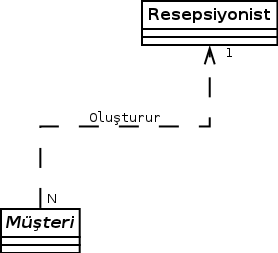
\includegraphics{dia/usecase1.png}
\end{center}

\newpage

\begin{center}
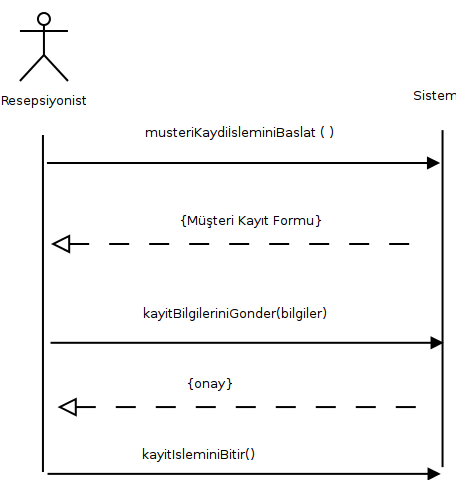
\includegraphics{dia/ssd-usecase1.png}
\end{center}

\newpage
\begin{description}
\item[Use Case 2:] Oda Kiralama \\
\item[Scope:] Otel Rezervasyon Sistemi
\item[Level:] User Goal
\item[Primary Actor:] Resepsiyonist 
\item[Stakeholders and Interests:] \hspace{10 mm}
\begin{description} 
\item[Resepsiyonist:] Oda kiralama işleminin her şeyiyle birlikte sorunsuz ve kolayca yapılabilmesini bekler
\item[Müşteri:] Oda kiralama işleminin yapılmasını bekler.
\item[Sistem Yöneticisi:] Oda kiralama işlemindeki bilgilerin eksiksiz olmasını bekler.
\end{description}
\item[Preconditions:] \hspace{10mm}
\begin{itemize}
\item Resepsiyonist sistemde kayıtlı ve yetkiye sahip olmalı.
\item Resepsiyonist sisteme giriş yapmış olmalı.
\item Sistemde en az bir otel olmalı.
\item Sistemde boş en az bir oda olmalı.
\item Müşteri sisteme kayıtlı olmalı.
\end{itemize}

\item[Postconditions:] \hspace{10mm}
\begin{itemize}
\item Oda kiralanmış ve müşteri ile ilişkilendirilmiş olmalı.
\end{itemize}
\item[Main Success Scenario (or Basic Flow):] \hspace{10mm}
\begin{enumerate}
\item Müşteri otele gelir ve resepsiyoniste talebini iletir.
\item Resepsiyonist müşteriden TC kimlik numarasını ister.
\item Resepsiyonist müşteriden kimliğini kanıtlanmasını talep eder.
\item Resepsiyonist TC kimlik numarasını yeni oda talebiyle birlikte sisteme girer.
\item Sistem yapılacak işlemi müşteri ile ilişkilendirir.
\item Sistem resepsiyoniste müşteriye uygun tipte boş odaları listeler.
\item Resepsiyonist müşteriye uygun odaları özellikleriyle belirtir ve bir seçim yapmasını bekler
\item Resepsiyonist seçilen odayı sisteme girer.
\item Resepsiyonist müşteriden kalacağı tarihleri talep eder ve sisteme girer.
\item Resepsiyonist bilgileri sisteme girer ve kayıt işlemini sisteme iletir.
\item Sistem toplam tahsil edilmesi gereken parayı gösterir.
\item Resepsiyonist parayı müşteriden tahsil eder ve sisteme iletir.
\item Sistem işlemin başarı ile gerçekleştiğini bildirir.
\end{enumerate}
\item[Extensions (or Alternative Flows):] \hspace{10mm}
\begin{itemize}
\item[*a] Senaryodaki herhangi bir ölümcül hatada:
    \begin{enumerate}
    \item Bütün işlemler ipyal edilip her şey baştan yazılır.
    \end{enumerate}
\item[3a] Müşteri kimliğini kanıtlayamaz ise 
    \begin{enumerate}
    \item Oda kayıt işlemi iptal edilir.
    \end{enumerate}
\item[6a] Müşteriye uygun oda yoksa:
    \begin{enumerate} 
    \item Müşteri bilgilendirilir.
    \item Kayıt işlemi tamamlanmadan iptal edilir.
    \end{enumerate}
\item[7a] Müşteri sunulan odalardan hiç birini beğenmezse.
    \begin{enumerate}
    \item İşlem tamamlanmadan iptal edilir
    \end{enumerate}
\item[9a] Müşterinin çıkış tarihinden önce oda rezarvasyon edilmişse
    \begin{enumerate}
    \item Sistem resepsiyoniste rezarvasyon yapılan tarihi gösterir
    \item Resepsiyonist müşteriyi bilgilendirir
    \item 6. adıma geri dönülür
    \end{enumerate}
\item[12a] Ödeme yapılmazsa
    \begin{enumerate}
    \item İşlem iptal edilir.
    \end{enumerate}
\end{itemize}
\end{description}

\begin{center}
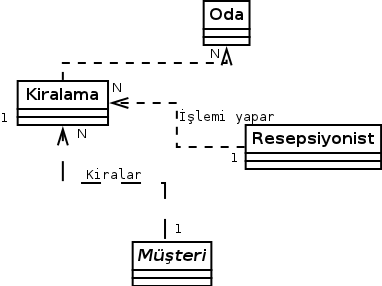
\includegraphics{dia/usecase2.png}
\end{center}

\begin{center}
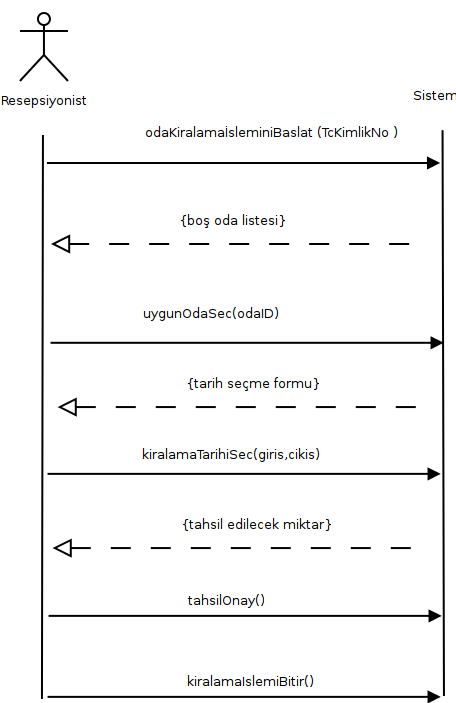
\includegraphics{dia/ssd-usecase2.png}
\end{center}

\newpage
\begin{description}
\item[Use Case 3:] Oda Ekleme \\
\item[Scope:] Otel Rezervasyon Sistemi
\item[Level:] User Goal
\item[Primary Actor:] Sistem Yöneticisi 
\item[Stakeholders and Interests:] \hspace{10 mm}
\begin{description} 
\item[Sistem Yöneticisi:] Odanın tanımlanması ile ilgili herhangi bir eksiklik olmamasını ister.
\end{description}
\item[Preconditions:] \hspace{10mm}
\begin{itemize}
\item Otel sistemde kayıtlı olmalı.
\item Sistem yöneticisi sisteme kayıtlı ve giriş yapmış olmalı.
\item Oda katologu sisteme kayıtlı olmalı.
\end{itemize}

\item[Postconditions:] \hspace{10mm}
\begin{itemize}
\item Oda rezervasyona hazır olmalı
\end{itemize}
\item[Main Success Scenario (or Basic Flow):] \hspace{10mm}
\begin{enumerate}
\item Sistem yöneticisi oda eklemek için yeni bir işlem başlatır.
\item Sistem uygun oda kataloglarını sistem yöneticisine listeler
\item Sistem yöneticisi ugun kataloğu seçer
\item Sistem odanın diğer özelliklerinin girilmesi için gerekli ekranı sunar
\item Odanın numarasını ve diğer özelliklerini sisteme girer.
\item İşlem tamamlanır.
\end{enumerate}
\item[Extensions (or Alternative Flows):] \hspace{10mm}
\begin{itemize}
\item[*a] Senaryodaki herhangi bir ölümcül hatada:
    \begin{enumerate}
    \item Bütün işlemler ipyal edilip her şey baştan yazılır.
    \end{enumerate}
\item[5a] Aynı numaralı başka bir oda varsa:
    \begin{enumerate}
    \item Sistem yöneticiden başka bir oda numarası ister.
    \item Eşsiz bir oda numarası girilinceye kadar 5a tekrarlanır.
    \item İşlem kaldığı yerden devam eder.
    \end{enumerate}
\end{itemize}
\end{description}
\begin{center}
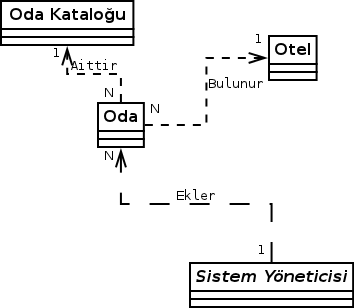
\includegraphics{dia/usecase3.png}
\end{center}

\newpage

\begin{center}
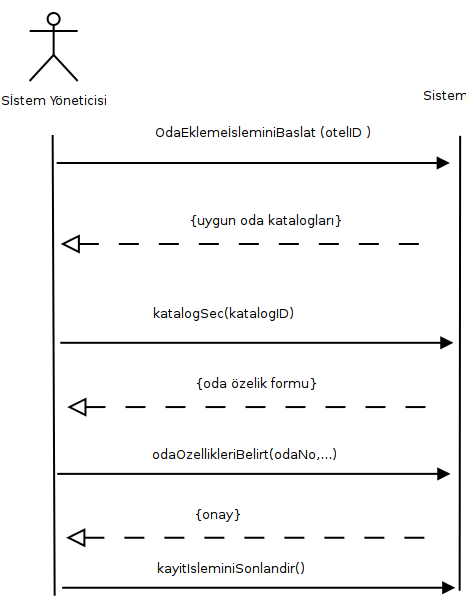
\includegraphics{dia/ssd-usecase3.png}
\end{center}

\newpage
\begin{description}
\item[Use Case 4:] Otel Ekleme \\
\item[Scope:] Otel Rezervasyon Sistemi
\item[Level:] User Goal
\item[Primary Actor:] Sistem Yöneticisi 
\item[Stakeholders and Interests:] \hspace{10 mm}
\begin{description} 
\item[Sistem Yöneticisi:] Otelin özelliklerinin doğru tanımlanmış olmasını bekler.
\end{description}
\item[Preconditions:] \hspace{10mm}
\begin{itemize}
\item Sistem yöneticisi sisteme kayıtlı ve giriş yapmış olmalı.
\end{itemize}

\item[Postconditions:] \hspace{10mm}
\begin{itemize}
\item Otel sisteme tüm özellikleri ile kaydedilmiş olmalı.
\end{itemize}
\item[Main Success Scenario (or Basic Flow):] \hspace{10mm}
\begin{enumerate}
\item Sistem yöneticisi yeni bir otel kaydı başlatır.
\item Otel için gerekli bilgiler istenir.
\item Sistem yöneticisi gerekli bilgileri girer.
\item Kayıt işlemi tamamlanır.
\end{enumerate}
\item[Extensions (or Alternative Flows):] \hspace{10mm}
\begin{itemize}
\item[*a] Senaryodaki herhangi bir ölümcül hatada:
    \begin{enumerate}
    \item Bütün işlemler iptal edilip her şey baştan yazılır.
    \end{enumerate}
\item[2a.] Aynı isimli başka bir otel varsa
    \begin{enumerate}
    \item Sistem yeni bir otel ismi girilmesini ister.
    \item Eşsiz bir otel ismi girilene kadar 2a devam eder.
    \item İşleme kalınan yerden devam edilir.
    \end{enumerate}
\item[2b.]
    \begin{enumerate}
    \item Sistem yeni bir adres girilesini ister.
    \item Eşsiz bir adres girilene kadar 2a devam eder.
    \item İşleme kalınan yerden devam edilir.
    \end{enumerate}
\end{itemize}
\end{description}

\begin{center}
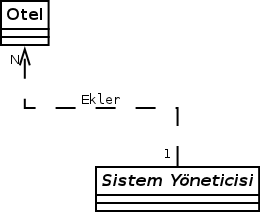
\includegraphics{dia/usecase4.png}
\end{center}

\newpage

\begin{center}
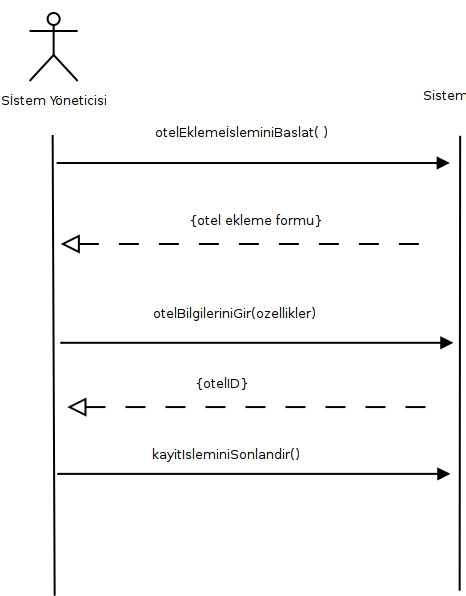
\includegraphics{dia/ssd-usecase4.png}
\end{center}

\newpage
\begin{description}
\item[Use Case 5:] Resepsiyonist Ekleme\\
\item[Scope:] Otel Rezervasyon Sistemi
\item[Level:] User Goal
\item[Primary Actor:] Sistem Yöneticisi 
\item[Stakeholders and Interests:] \hspace{10 mm}
\begin{description} 
\item[Sistem Yöneticisi:] Yeni bir resepsiyonistin sisteme kayıtlı olmasını bekler.
\end{description}
\item[Preconditions:] \hspace{10mm}
\begin{itemize}
\item Sistem yöneticisi sisteme kayıtlı ve giriş yapmış olmalı
\end{itemize}

\item[Postconditions:] \hspace{10mm}
\begin{itemize}
\item Resepsiyonist sisteme kaydedilmiş olmalı.
\end{itemize}
\item[Main Success Scenario (or Basic Flow):] \hspace{10mm}
\begin{enumerate}
\item Sistem yöneticisi yeni bir resepsiyonist kaydı başlatır.
\item Sistem resepsiyonist için gerekli bilgileri ister.
\item Sistem yöneticisi gerekli bilgileri girer.
\item Kayıt işlemi tamamlanır.
\end{enumerate}
\item[Extensions (or Alternative Flows):] \hspace{10mm}
\begin{itemize}
\item[*a] Senaryodaki herhangi bir ölümcül hatada:
    \begin{enumerate}
    \item Bütün işlemler ipyal edilip her şey baştan yazılır.
    \end{enumerate}
\item[2a] Aynı kullanıcı isimli başka bir resepsiyonist varsa
    \begin{enumerate}
    \item Sistem yeni bir kullanıcı adı girilmesini ister.
    \item Eşsiz bir isim girilene kadar 2a devam eder.
    \item İşlem kaldığı yerden devam eder.
    \end{enumerate}
\end{itemize}
\end{description}

\begin{center}
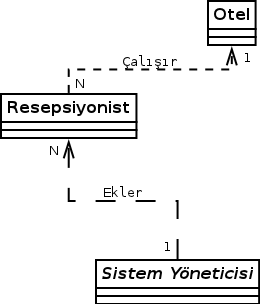
\includegraphics{dia/usecase5.png}
\end{center}

\newpage

\begin{center}
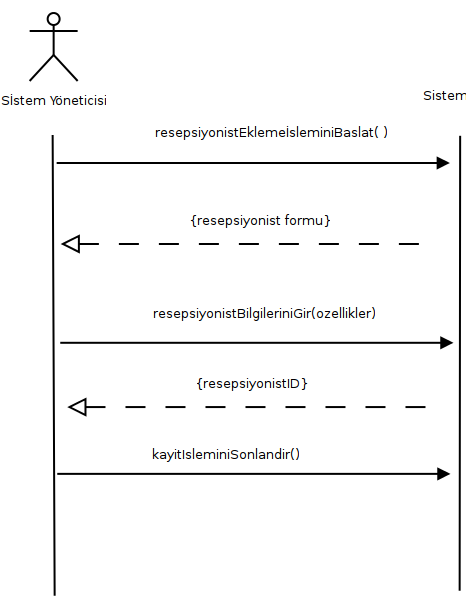
\includegraphics{dia/ssd-usecase5.png}
\end{center}

\newpage
\begin{description}
\item[Genel Domain UML Diagramı: ] \hfill

\end{description}

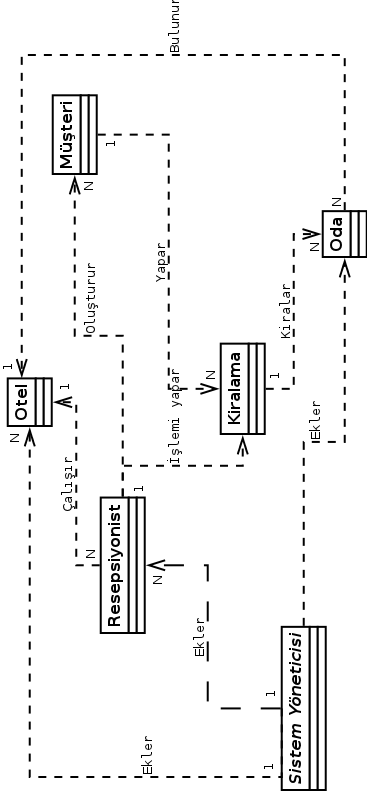
\includegraphics{dia/allusecasessmall.png}


\end{document}
